\documentclass[floatfix,twocolumn,prl,showpacs,preprintnumbers,amsmath,nofootinbib,amssymb,noeprint,superscriptaddress]{revtex4-1}
\usepackage[utf8]{inputenc}
\setcounter{secnumdepth}{1}
\usepackage{comment}
\usepackage{bm}
\usepackage[pdftex]{color}
\usepackage{xcolor}
\usepackage{graphicx,capt-of}
\usepackage{amsmath,amssymb,amsfonts,mathtools}
\usepackage{braket}
\usepackage[colorlinks=true,linkcolor=black,filecolor=black,urlcolor=blue,citecolor=blue,pdftex,plainpages=false]{hyperref}
\newcommand{\blue}[1]{{\color{blue} #1}}
\newcommand{\nn}{\nonumber}
\usepackage{ulem}
\newcommand{\fourpt}{{4\mathrm{pt}}}
\newcommand{\twopt}{{2\mathrm{pt}}}
\newcommand{\Op}{\mathcal{O}}
\newcommand{\Opbar}{\overline{\Op}}
\newcommand{\tr}{\operatorname{tr}}
\newcommand{\dd}{\mathrm{d}}

%%%%%%%%%%%%%%%%%%%%%%%%%%%%%%%%%%%%%%%%

\newcommand{\red}{\textcolor{red}}
\newcommand{\RZ}[1]{{\color{blue} [RZ: #1]}}
\newcommand{\CZ}[1]{{\color{orange} [CZ: #1]}}
\newcommand{\ZJL}[1]{{\color{brown} [ZJL: #1]}}

\begin{document}
\preprint{MIT-CTP/6027}

\title{Parton Distribution Functions from Large Momentum Expansion \\ of Current-Current Correlators}

\author{Jialu Zhang}
\affiliation{Tsung-Dao Lee Institute and School of Physics and Astronomy, Shanghai Jiao Tong University, Shanghai 201210, China}
\author{Xiangdong Ji}
\affiliation{Tsung-Dao Lee Institute and School of Physics and Astronomy, Shanghai Jiao Tong University, Shanghai 201210, China}
\affiliation{Department of Physics, University of Maryland, College Park, MD 20742, USA}
\author{Andreas Sch\"afer}
\affiliation{Institute for Theoretical Physics, University of Regensburg, 93040 Regensburg, Germany}
\author{Rui Zhang}
\email{rzhang93@mit.edu,corresponding author}
\affiliation{Center for Theoretical Physics - a Leinweber Institute, Massachusetts Institute of Technology, Cambridge, MA 02139, USA}
\author{Christian Zimmermann}
\email{chrzim@lbl.gov,corresponding author}
\affiliation{Department of Physics and Astronomy, University of Kentucky, Lexington, KY 40506, USA}
\affiliation{Nuclear Science Division, Lawrence Berkeley National Laboratory, Berkeley, CA 94720, USA}
\begin{abstract}
The universality of the large momentum expansion allows computing parton distribution functions (PDFs) starting from any Euclidean correlator with appropriate large momentum Fourier Components. Here we consider current-current correlators which have been used 
in short-distance expansion to obtain moments of PDFs. The advantage 
of such correlators is that they have simple renormalization
properties and do not have linear power divergences as in quasi-PDF.
However, in lattice calculations, four-point functions are needed. 
Here we present an expansion formula with current-current correlators
up to the next-to-leading order, and preliminary numerical calculations
with four-point functions.
\end{abstract}

\maketitle
\text{\it Introduction:}
Parton distribution functions (PDFs) are fundamental quantities in quantum chromodynamics (QCD) that describe the hadronic structure in terms of quark and gluon degrees of freedom on the light cone. They are universal inputs to the prediction of hadronic processes at, e.g., the LHC~\cite{ATLAS:2019mfr} and the upcoming Electron-Ion Collider (EIC)~\cite{Accardi:2012qut,AbdulKhalek:2021gbh}, and can be determined from global fitting to experimental data.
Meanwhile, it is also interesting to theoretically calculate these observables non-perturbatively from first-principle lattice QCD. While there are fundamental difficulties to fully extract these light-like observables on a Euclidean lattice, large momentum effective theory (LaMET)~\cite{Ji:2013dva,Ji:2014gla} provides a framework to directly calculate the mid-range Bjorken-$x$ dependence of PDFs through the large momentum expansion of Euclidean correlations. Various other approaches have also been proposed to extract partial information on PDFs from lattice QCD, which can be found in recent reviews~\cite{Lin:2017snn,Cichy:2018mum,Constantinou:2020pek,Constantinou:2020pek,Constantinou:2022yye,Lin:2025hka}.

The LaMET framework introduces a universality class of distributions~\cite{Ji:2020ect}. The leading order expansion of these distributions in terms of $(\Lambda_{\rm QCD}/P_z)$ contains the same infrared (IR) structure as the lightcone PDFs, thus can be perturbatively matched to them. The simplest member of this universality class is the quasi-PDF, which is the Euclidean version of the lightcone correlation function, and can be interpreted as the physical momentum distribution of quarks and gluons in a hadron with finite momentum. Other variants in the same universality class include the Coulomb gauge distributions proposed recently~\cite{Gao:2023lny,Zhao:2023ptv} and the current-current correlations~\cite{Ji:2020ect}. Since the proposal of LaMET, significant theoretical improvements have been developed to better control the systematics for the quasi-PDF calculations in the past decade~\cite{Ji:2017oey,Ishikawa:2017faj,Green:2017xeu,Constantinou:2017sej,Stewart:2017tvs,Alexandrou:2017huk,Izubuchi:2018srq,Li:2020xml,Chen:2020ody,Ji:2020brr,Gao:2021hxl,LatticePartonLPC:2021gpi,Su:2022fiu,Zhang:2023bxs,Ji:2023pba,Liu:2023onm,Ji:2024hit,Chen:2025cxr,Ji:2026vir}. One challenge of the precision PDF calculation from quasi-PDFs is the renormalization of the ultraviolet (UV) divergence in the Wilson-line self energy~\cite{Chen:2016fxx,Green:2017xeu,Ji:2017oey,Ishikawa:2017faj,Ji:2020brr}. Coulomb gauge distributions avoid this issue by not including the spatial Wilson line in the operator, and have demonstrated advantages in numerical precision in the calculation of the transverse-momentum-dependent  observables~\cite{Gao:2023lny,Zhao:2023ptv}, but their factorization has not been proved at all orders. The LaMET calculation using current-current correlations does not have a renormalization issue and is well understood in theory, but has not been studied because it requires the more expensive measurements of four-point correlation functions on the lattice.

Current-current correlations have attracted a lot of interest due to their close relation to physical cross sections in collider physics. Various methods of extracting PDFs from current-current correlations has been proposed, including the hadronic tensor~\cite{Liu:1999ak}, the ``Ioffe time'' distributions~\cite{Braun:2007wv}, the Compton amplitude~\cite{Chambers:2017dov}, and the ``lattice cross sections''~\cite{Ma:2017pxb}. They can also be studied to understand the twist-4 double-parton distributions~\cite{Diehl:2011yj}. As the availability of computational resources develops, these calculations now become routinely feasible, and some first lattice calculations have been realized in recent years~\cite{Chambers:2017dov,Bali:2018spj,Liang:2019frk,Sufian:2020vzb,Bali:2021gel,Zimmermann:2024zde}. 
The common basis of these methods is the operator product expansion (OPE), which allows a short distance factorization (SDF) of the correlators into lightcone distributions and perturbative matching kernels when the two currents are separated by a perturbative Euclidean distance. They can extract moments of PDFs, or fit the data to some parametrization of the $x$-dependent PDFs.

As current-current correlations are also in the same universality class of distributions introduced by LaMET, lightcone PDFs can be factorized in terms of current-current correlations, and their $x$-dependence can be directly calculated through perturbative matching~\cite{Ji:2024oka}. The differences between SDF and LaMET applications of the similar lattice data are explained in Ref.~\cite{Ji:2022ezo}.

In this paper, we develop the $x$-space formulation for the large momentum expansion of the two-current matrix elements of vector (V) and axial vector (A) currents, and calculate the $x$-dependent PDFs in lattice QCD. For this first analysis, we re-use the current-current matrix element data generated in the context of a previous project. We show some first results for the proton PDF $f_{u-d}$, demonstrating the feasibility of the presented approach.


\text{\it Theory:}  
We start from forward matrix elements of two currents in the proton. We consider unpolarized matrix elements, i.e.\ we implicitly average over helicity states:

\begin{align}
    M_{XY,ab}^{\mu\nu}(z,P) 
    = 
    \bra{P}
    J^\nu_{X,ab}(z)\ 
    J^\mu_{Y,ba}(0)
    \ket{P} \,,
    \label{eq:Mdef}
\end{align}
%
where $J^\mu_{X,ab}(z)$ are local currents. Specifically, we consider two types: 

\begin{align}
    J^\mu_{\mathrm{V},ab}(z) 
    :=
    \bar{q}_a(z)\ \gamma^\mu\ q_b(z)
    \,,\nonumber\\
    J^\mu_{\mathrm{A},ab}(z) 
    :=
    \bar{q}_a(z)\ \gamma^\mu \gamma_5\ q_b(z) \,.
\end{align}
The indices $a$ and $b$ indicate the flavor of the quark field, with the index $a$ specifying the quark PDF under consideration. The singlet (non-singlet) contribution is defined for $b=a$ ($b\neq a$). We are free to select the flavor $b$, and the calculation simplifies drastically if we choose $b$ to be an (auxiliary) quark flavor that is different from the valence quark flavors of the considered hadron, in our case a proton. The spatial separation $z=(0,\vec{z})$ is chosen to be parallel to the direction of the proton's momentum $\vec{P}$ with $|\vec{P}|\gg\Lambda_{\rm QCD}$.
In the following, we discuss the current combination VV where we already have lattice data from previous work, the case AA works in an analog way. 
The leading contribution to the hadronic tensor is given by transverse polarizations, thus for arbitrary lattice momentum $\vec{P}=(P_x,P_y,P_z)$, the spin structure can be replaced with the following projection of Dirac matrices,

\begin{align}
    \Gamma^i=\sum_{i\in\{x,y,z\}}\left(\delta_{ij}-\frac{P_i P_j}{|\vec{P}|^2}\right)\gamma_j,
    \label{eq:transverse_proj}
\end{align}
%
where only two of them are independent, spanning the 2-dimensional transverse plane, such that $\Gamma\cdot \vec{P}=0$. We can further average the data on the transverse plane for the VV current by taking a trace, yielding
\begin{align}
M^{\perp\perp}_{\mathrm{VV},ab}&(z,P)
=\frac{1}{2}\sum_{i,j} \left(\delta_{ij}-\frac{P_iP_j}{|P|^2}\right)
M_{\mathrm{VV},ab}^{ij}(z,P)
\label{eq:Wperp}
\end{align}
%
Moreover, it is useful to define:

\begin{align}
    W^{\perp\perp}_{\mathrm{VV},ab}(z,P) 
    := 
    -\frac{i\pi^2 z^4}{\vec{z}\cdot\vec{P}}
    M^{\perp\perp}_{\mathrm{VV},ab}(z,P) \,,
    \label{eq:Wdef}
\end{align}
%
and likewise for the AA combination.   As explained in Ref.~\cite{Ma:2014jla}, these correlators exhibit the same infrared divergence structure as the PDFs. 
Therefore, their $x$-space conjugate can be used to calculate the PDFs through the LaMET approach. 
One of the most important merits of these correlators is that they are constructed from conserved vector and axial-vector currents and do not involve Wilson lines. As a result, no UV divergence arises at one-loop order, and the correlators are free from power UV divergences and UV renormalon ambiguities.

As we shall explain later in this work, we average the matrix elements of the VV and AA currents,

\begin{align}
    W^{\perp\perp}(z,P)=\frac{1}{2}\left(	W^{\perp\perp}_{\mathrm{VV}}(z,P)+	W^{\perp\perp}_{\mathrm{AA}}(z,P)\right),
    \label{eq:VVAA-combo}
\end{align}
%
and obtain the momentum-space VV-distribution through the Fourier transform,

\begin{align}
\tilde{h}(y,P_z)
&=
\int_{-\infty}^\infty \frac{P_z\dd z}{2\pi}\,
e^{i y zP_z}\,
W^{\perp\perp}\!\left(z,P\right).
\end{align}
The light-cone PDF can be factorized into the VV-distribution and perturbative matching~\cite{Ji:2024oka},

\begin{align}
\label{eq:lm_expansion}
f(x,\mu^2)
=
\int_{-\infty}^{\infty} \frac{\dd y}{|y|}\,
C\!\left(\frac{x}{y},\frac{|y|P_z}{\mu}\right)
\, \tilde{h}(y,P_z)
+ ...\, ,
\end{align}
%
where $C\!\left(\frac{x}{y},\frac{|y|P_z}{\mu}\right)$ is the matching kernel calculable in
perturbation theory, and the higher twist contributions in the expansion parameter $\mathcal{O}\left(\frac{\Lambda^n_{\rm QCD}}{(xP_z)^n},\frac{\Lambda^n_{\rm QCD}}{((1-x)P_z)^n},\frac{M^n}{P_z^n}\right)$ are omitted for $n\geq2$. In this way, LaMET provides a forward matching
that enables a direct determination of PDFs from lattice-computable
quasi-distributions, with systematically improvable power corrections suppressed by inverse powers of $P_z$.

We calculate the perturbative matching kernel up to one loop in the $\overline{\text{MS}}$ scheme, with the \text{\it naive dimensional regularization}, where the VV and AA are exactly the same at one loop order. Thus we have,
\begin{widetext}
\begin{equation}\label{eq:matching}
\begin{aligned}
C_{\rm ns}^{\overline{\text{MS}}}\bigg(\xi,\frac{|y|P_z}{\mu}\bigg)=&\delta(1-\xi)+\frac{\alpha_s C_F}{4\pi}\delta(1-\xi)\\
&+\frac{\alpha_s C_F}{2\pi}
\begin{cases}
\bigg[\frac{\left(\xi ^2+1\right) \log \left(\frac{\xi -1}{\xi }\right)+\xi +1/2 }{ 1-\xi}\bigg]_{+(1)}^{[1,\infty)} & \text{if } \xi>1 \\[6pt]
\bigg[\frac{2 \left(\xi ^2+3\right) \log (1-\xi )+2 \left(\xi ^2+1\right) \log (\xi )+2 (\xi -4) \xi +7}{2 (\xi -1)}\bigg]_{+(1)}^{[0,1]}+ \bigg[\frac{1+\xi^2}{1-\xi}\bigg]_{+(1)}^{[0,1]}\log\big(\frac{\mu^2}{4y^2P_z^2}\big) & \text{if } 0<\xi<1\\[6pt]
\bigg[\frac{ \left(\xi ^2+1\right) \log \left(\frac{\xi -1}{\xi }\right)+ \xi +1/2}{ (\xi -1)}\bigg]_{+(1)}^{(-\infty,0]}& \text{if } \xi<0
\end{cases}
\end{aligned}
\end{equation}
\end{widetext}
%
where $\xi=\frac{x}{y}$, and the plus distribution is defined as

\begin{align}
\int_D \dd x \, [g(x)]^{D}_{+(x_0)} \, h(x)
=
\int_D \dd x \, g(x)\,[h(x)-h(x_0)] \, .
\end{align}
%
The PDFs can also be calculated from the VA or AV correlations, which have been studied before for the pion valence PDF in the short-distance factorization framework~\cite{Sufian:2020vzb}. We can obtain the VA matrix elements through (assuming $x,y$ to be two transverse directions),

\begin{align}
    W^{\perp\perp}_{\mathrm{VA}}:=\frac{\pi^2z^3}{2E_P}
&\left[
M^{xy}_{\mathrm{VA}}(z,P)
+
M^{xy}_{\mathrm{AV}}(z,P)
\right]\,,
\end{align}
%
where $E_P = \sqrt{\vec{P}^2 + m^2}$ is the proton energy.
The corresponding matching kernel needs an extra correction term compared to Eq.~\eqref{eq:matching},

\begin{align}
    C_{\rm VA, ns}^{\overline{\text{MS}}}(\xi)=C_{\rm ns}^{\overline{\text{MS}}}(\xi)+\frac{\alpha_sC_F}{\pi}[1-\xi]_{+(1)}^{[0,1]}\theta(\xi)\theta(1-\xi)\,.
\end{align}

\text{\it Simulation details:}
In this first analysis, we re-use the two-current matrix elements that have already been produced in the context of other simulations \cite{Bali:2021gel} employing the $n_f=2+1$ Wilson-Clover gauge ensembles provided by the CLS collaboration \cite{Bruno:2014jqa}. Specifically, we use the ensemble H102 with extension $32^3\times 96$, lattice spacing $a=0.085~\mathrm{fm}$, and pion mass $m_\pi=355~\mathrm{MeV}$. The matrix element in \eqref{eq:Mdef} can be calculated on the lattice in Euclidean spacetime if the separation between the two currents is purely spatial. The  matrix elements can then be expressed in terms of a Euclidean four-point correlation function in the limit of large time separations to suppress excited state contributions:

\begin{align}
    M^{\mu\nu}(z,P)
    =
    E_P V
    \left.
    \frac{C^{\mu\nu}_{\fourpt}(\vec{P},\vec{z},\tau,t)}{C_{\twopt}(\vec{P},t)}
    \right|_{0\ll\tau\ll t} \,,
    \label{eq:M-ratio}
\end{align}
%
where the four-point function reads

\begin{align}
    &C^{\mu\nu}_{\fourpt}(\vec{P},\vec{z},\tau,t)
    \nonumber\\
    &\quad:=
    \left\langle
    \Op^{\vec{P}}(t)\ 
    J_{ab}^\mu(\vec{z},\tau)\ 
    J_{ba}^\nu(\vec{0},\tau)\ 
    \Opbar^{\vec{P}}(0)
    \right\rangle \,.
    \label{eq:4ptdef}
\end{align}
%
\begin{figure}[tb]
    \centering
    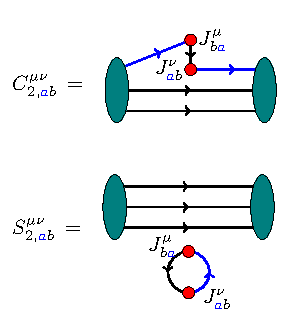
\includegraphics[width=0.6\columnwidth]{graphs_t0_ns.pdf}
    \caption{Wick contractions that can contribute to the four-point correlation function \eqref{eq:4ptdef} in the case of an auxiliary intermediate quark field of flavor $b$. Flavor $a$ (blue) specifies the PDF.}
    \label{fig:graphs}
\end{figure}
%
$C_{\twopt}$ is the usual two-point function, $E_P = \sqrt{\vec{P}^2 + m^2}$ the proton energy, and $V$ is the spatial lattice volume. The operators $\Op^{\vec{P}}$, $\Opbar^{\vec{P}}$ respectively annihilate or generate the desired hadron, in our case, the proton. In general, there are several types of Wick contractions that can contribute to \eqref{eq:4ptdef} as has been worked out in detail in \cite{Bali:2021gel}. As already mentioned, we consider $b$ to be different from the flavors of the valence quarks in the considered hadron (non-singlet contribution). In this case, only the contractions $C_2$ and $S_2$ shown in Fig. \ref{fig:graphs} contribute. The latter represents a pure sea quark contributions. In the current analysis, we restrict ourselves to the isovector PDF, i.e.\ $f_{u-d}$, where the $S_2$ contributions cancel. Hence, we only have to evaluate the contraction $C_2$. The methods and techniques to evaluate the required diagrams have been worked out in \cite{Bali:2021gel}. 

In this work, we only give a brief summary for the required diagram $C_2$: We use a momentum smeared source \cite{Bali:2016lva} to obtain a point-to-all propagator. The sink is realized using the sequential source technique again employing momentum smearing.
The propagator between the two currents is evaluated using the stochastic source technique, which is accompanied by improvements exploiting the hopping parameter expansion for Wilson fermions. This allows us to efficiently calculate the matrix element \eqref{eq:M-ratio} for all current separations $\vec{z}$. The data currently used were produced using 96 stochastic sources. As discussed in \cite{Zimmermann:2024zde}, the contribution of the $C_2$ diagram is sensitive to discretization artifacts of the Wilson propagator. In part, this is due to a non-vanishing chiral odd contribution to the Wilson propagator. This is avoided by taking combinations of Dirac structures where these chiral odd contributions cancel, e.g.\ the combination $(M_{VV}+M_{AA})/2$ given in \eqref{eq:VVAA-combo} \cite{Bali:2018spj,Zimmermann:2024zde}. The remaining anisotropy artifacts are suppressed by performing a simple tree-level improvement where we multiply our data by the correction factor:

\begin{align}
    c^{\mathrm{corr}}(z) 
    =
    \frac{\tr\left\{ z\!\!\!/ M^{\mathrm{free}}_{\mathrm{cont}}(z) \right\}}{\tr\left\{ z\!\!\!/ M^{\mathrm{free}}_{\mathrm{latt}}(z) \right\}}
    = 
    -\frac{m^2}{\pi^2} \frac{K_2(m\sqrt{-z^2}) }{ \tr\left\{ z\!\!\!/ M^{\mathrm{free}}_{\mathrm{latt}}(z) \right\} }
\end{align}
%
In order to keep the systematic uncertainties associated with this kind of improvement small, it is advisable to restrict to data points where $c^{\mathrm{corr}}(z)$ is close to 1. In past studies, it has been found  that this is mainly the case if $\vec{z}$ is in the vicinity of one of the lattice diagonals \cite{Bali:2018spj,Zimmermann:2024zde}. The simulation is carried out for proton momenta of the form $(\pm n,\pm n,\pm n)$ so that $\vec{z}$ is indeed aligned with one of the lattice diagonals if one maximizes the scalar product $\vec{P}\cdot \vec{z}$, which is preferred in our LaMET calculation. At the moment, the largest available proton momentum is $|\vec{P}|_{\mathrm{max}} = \sqrt{12}\cdot 2\pi/L = 1.57~\mathrm{GeV}$. 


To maximally utilize the lattice data we have measured, we also include more data points when $\vec{P}$ and $\vec{z}$ are not perfectly aligned, and also other relevant Lorentz components in addition to the pure transverse operators. It increases the effective statistics of the measurement, and allows a smoother interpolation in coordinate space and a more stable Fourier transformation to $x$-space. To extract $M^{\perp\perp}$, we exploit the fact that $M^{\mu\nu}$ is a Lorentz-covariant object and decompose it in the case of $M_{VV}$ and $M_{AA}$ into the Lorentz structure:

\begin{align}
    &M^{\mu\nu}(z,P)
    =
    \frac{P^\mu P^\nu}{m^2} A(\lambda,z^2)
    -
    g^{\mu\nu} B(\lambda,z^2)
    \nonumber\\
    &\quad+
    m^2 z^\mu z^\nu C(\lambda,z^2)
    +
    (P^\mu z^\nu + P^\nu z^\mu) D(\lambda,z^2)\,.
    \label{eq:Ldecomp}
\end{align}
%
$M^{\perp\perp}$ is equivalent to the function $B$, which can be extracted by solving the over-determined system of equations given by the decomposition \eqref{eq:Ldecomp} taking into account all available data points of $M^{\mu\nu}(z,P)$ while maximizing statistics. $B$ is accessible for $-|\vec{P}|_{\mathrm{max}}|\vec{z}| \le \lambda \le |\vec{P}|_{\mathrm{max}}|\vec{z}|$. 
%\sout{Instead of fixing $P_z$ to the momentum the interpolators are projected onto, one can rather \textit{define} it as the ratio $P_z \equiv \lambda/|\vec{z}|$, which ensures that $\vec{P}$ and $\vec{z}$ are indeed aligned as required by the LaMET setup. This allows us to access multiple values of $P_z$ and obtain more data points as if we would have fixed $P_z$ in the conventional way. Since we expect $B$ to be a smooth function in $\lambda$, we allow a small tolerance of $2\%$ w.r.t.\ $P_z$, i.e.\ $P_z(1-0.02) \le \lambda/|\vec{z}| \le P_z(1+0.02)$, in order to take into account more data points.} 
By definition, the actual $P_z$ is now $P_z=\lambda/|\vec{z}|$ when $\vec{z}$ is not aligned to $\vec{P}$. To avoid a large logarithmic correction from combining data at different $P_z$, we only allow a small tolerance of $2\%$ w.r.t.\ $|\vec{P}|$, i.e.\ $|\vec{P}|(1-0.02) \le \lambda/|\vec{z}| \le |\vec{P}|(1+0.02)$.
%\CZ{I think the following is better: To avoid a large logarithmic correction from combining data at different $P_z$, we \textit{only} allow a small tolerance of...}\RZ{updated. Also I already mentioned ``$\vec{P}$ and $\vec{z}$ are not perfectly aligned'' in the previous paragraph, so I omitted it here.}

\text{\it Lattice Results:}
The lattice results for $W^{\perp\perp}_{u-d}$ are shown in 
Fig.~\ref{fig:raw_data} as functions of $z$. Given the current level of statistics, the real part matrix elements becomes consistent with zero at around $z\approx 0.42$ fm. For the moment, we employ a suitable ansatz for extrapolating the large-$z$ behavior. This generates some systematic uncertainty, which should be suppressed by improved data quality at large $z$ in future simulations.
The matrix element at $z=0$ is not directly accessible in lattice 
simulations because of the contact singularity. However, since the 
current-current operator is free of ultraviolet divergences, the 
corresponding $z=0$ value can be calculated perturbatively. In the 
$\overline{\mathrm{MS}}$ scheme, one finds 

\begin{align}
    W^{\perp\perp}(0,P)
    =
    1-\frac{\alpha_sC_F}{4\pi},
    \label{eq:Wdef}
\end{align}
%
which can then be consistently included in the Fourier transform.

\begin{figure}[tb]
    \centering
    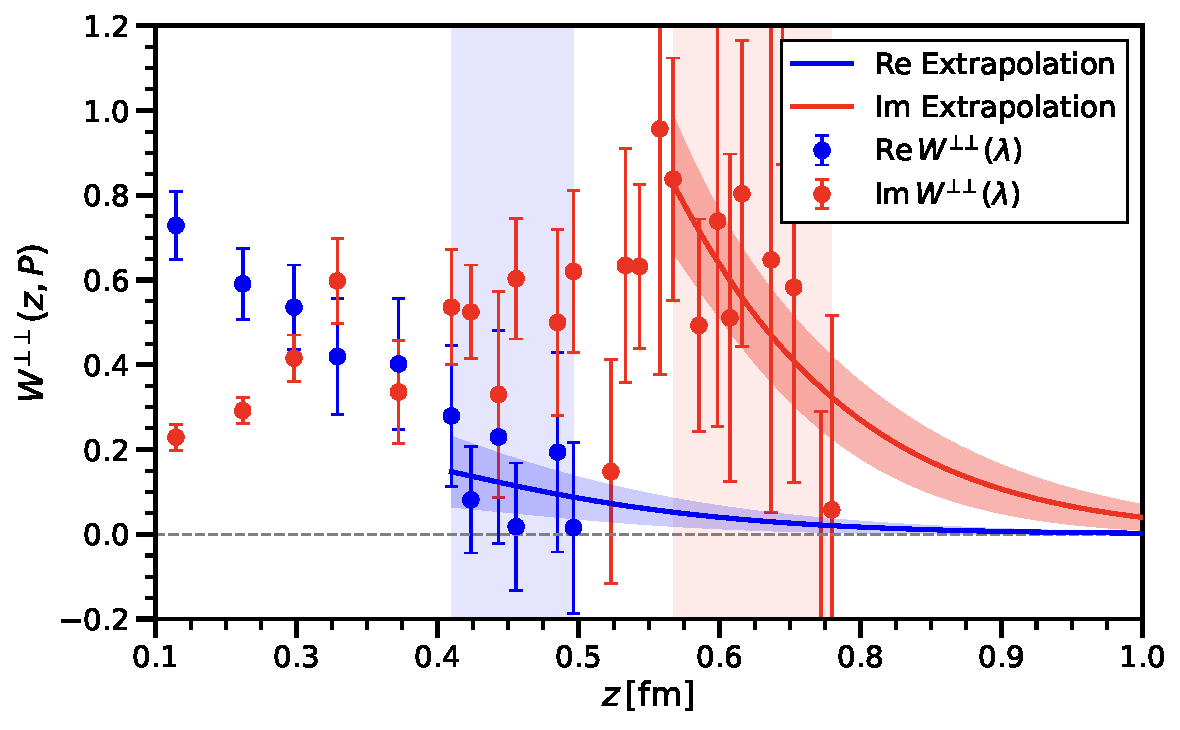
\includegraphics[width=\columnwidth]{raw_data_z.pdf}
    \caption{Real (red) and imaginary (blue) parts of 
    $W^{\perp\perp}_{u-d}$ as a function of $z$ from lattice simulation at 
    $|\vec{P}| = 1.523~\mathrm{GeV}$.}
    \label{fig:raw_data}
\end{figure}

To carry out the Fourier transform, we adopt an extrapolation ansatz 
for the large-$|z|$ region, motivated by its asymptotic behavior derived in Ref.~\cite{Ji:2026vir}. 
Specifically, we parameterize the correlator as
\begin{equation}
    W^{\perp\perp}(z,P)=A\,|z|^{5/2}e^{i\phi\,\mathrm{sign}(z)}e^{-m|z|},
\end{equation}
%
where $A$, $\phi$ and $m$ are fitting parameters.
The extrapolation ansatz is used in the Fourier transform starting from the point where the lattice data become dominated by noise. This happens for $z=0.51~\mathrm{fm}$ for the real part and $z=0.75~\mathrm{fm}$ for the imaginary part. With this choice, the dominant uncertainty remains statistical rather than the model dependence of the extrapolation.
Using this extrapolation together with the perturbative input at $z=0$, 
we obtain the momentum-space distribution $h(y,P_z)$ shown in 
Fig.~\ref{fig:hy}. Significant oscillations occur for outside the physical 
region, reflecting both the limited precision of the present lattice 
data and the residual uncertainty associated with the large-$|z|$ 
extrapolation.

\begin{figure}[tb]
    \centering
    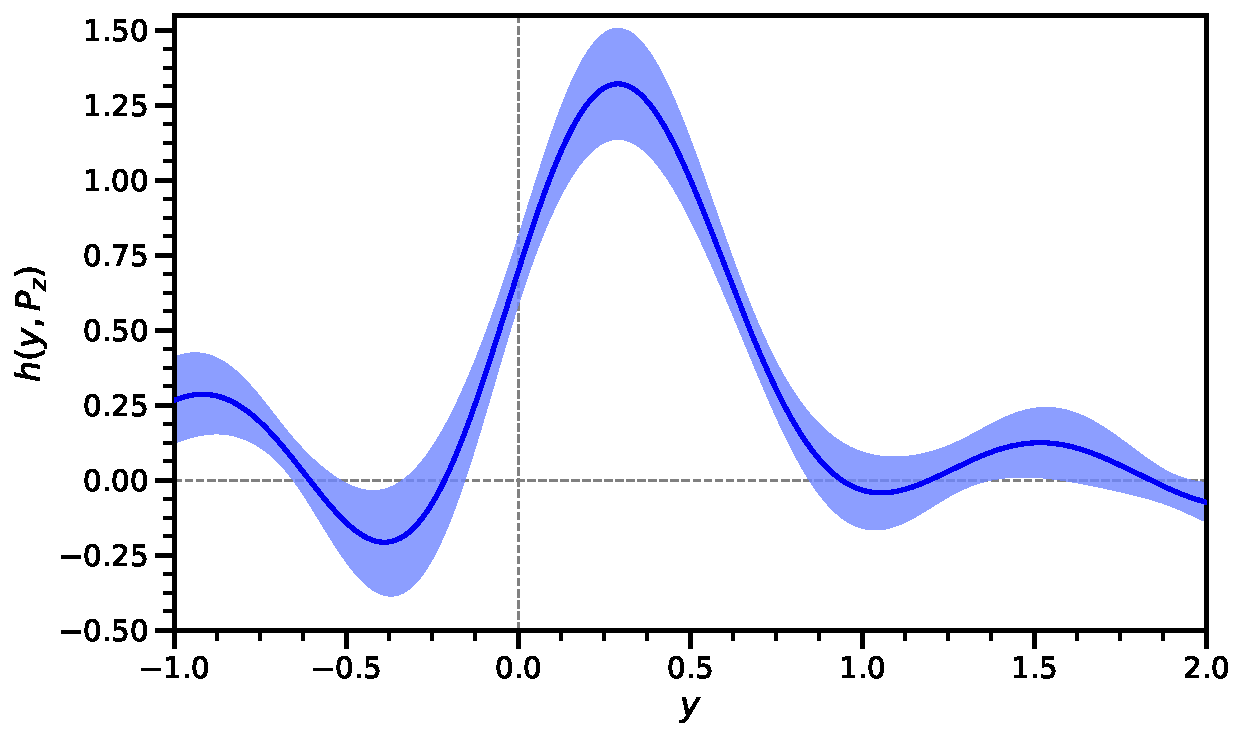
\includegraphics[width=\columnwidth]{hy.pdf}
    \caption{The momentum-space VV distribution $h(y,P_z)$ obtained 
    from lattice simulation at $|\vec{P}| = 1.523~\mathrm{GeV}$, shown 
    as a function of the momentum fraction $y$.}
    \label{fig:hy}
\end{figure}
%
After applying the matching formula in Eq.~(\ref{eq:lm_expansion}), and also following the renormalization group resummation (RGR) procedure proposed in Ref.~\cite{Su:2022fiu},  the 
resulting isovector PDF is shown in Fig.~\ref{fig:compare}, 
together with the CT18NNLO global-fit result. A noticeable deviation 
is observed. This is expected to be improved with larger hadron momenta, at which the parton's momentum will shift to smaller $x$. We emphasize that the present analysis with limited precision and hadron momentum is not intended to provide an 
accurate determination. Rather, it aims to demonstrate a feasible method 
for extracting PDFs from lattice QCD. 

\begin{figure}[tbp]
    \centering
    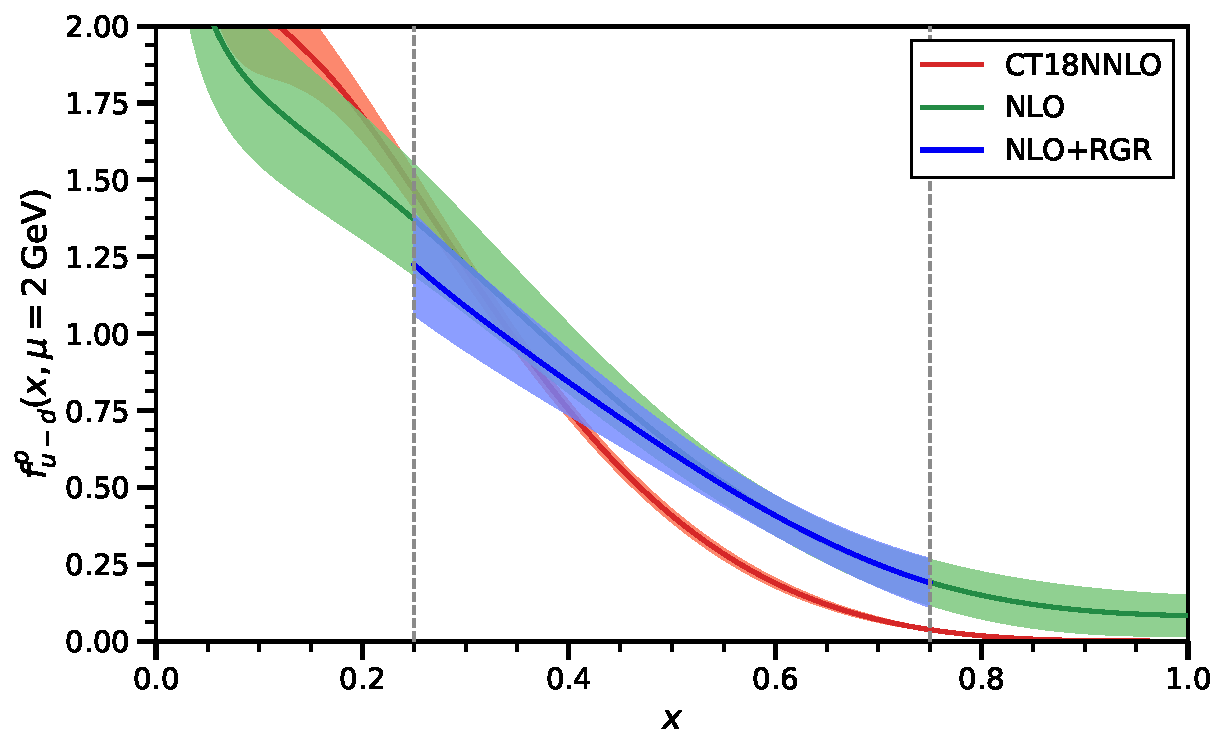
\includegraphics[width=\columnwidth]{pdf_rgr_shaded.pdf}
    \caption{The flavor non-singlet PDF $f_{u-d}(x,\mu)$ at 
    $\mu=2~\mathrm{GeV}$. The blue band shows the result obtained in 
    this work, while the red band denotes the CT18NNLO global-fit 
    result.}
    \label{fig:compare}
\end{figure}

\text{\it Conclusion:} We formulated a large momentum expansion of two-current matrix elements of two vector or two axial vector currents in order to calculate the $x$-dependence of the proton PDF. 
This first analysis was carried out for $f_{u-d}$, avoiding disconnected diagrams. This work provides a proof of concept of using current-current correlations in the framework of LaMET, which has several conceptual advantages compared to the conventional approach using Wilson-line operators, such as the absence of renormalon ambiguities. 
Notice that our analysis was carried out at a maximal proton momentum $|\vec{P}|=1.523~\mathrm{GeV}$ due to limitations in the availability of lattice data, which we re-used from a previous project that was not designed for performing a LaMET calculation. 
Moreover, the pion mass $m_\pi = 355~\mathrm{MeV}$ of the employed ensemble is higher than the physical one. This is in all probability the origin of the discrepancies between our lattice results and the experimental ones. In fact, as the hadron momentum increases, the partons are expected to migrate from large to small $x$ regions.
The next step will be to repeat the calculations for higher momenta ($|\vec{P}| > 2~\mathrm{GeV}$) at reasonably high statistics. 
In this context, the usage of the newly proposed kinematically enhanced interpolators \cite{Zhang:2025hyo} will be very helpful.  We leave this calculation for future work.

\section*{Acknowledgments}

We thankfully acknowledge the CLS effort for generating the $n_f = 2 + 1$ ensembles in \cite{Bruno:2014jqa}, one of which was used for this work. J.~Z. is supported by the T.~D.~Lee Scholarship. R.~Z. is partially supported by the U.S. Department of Energy, Office of Science, Office of Nuclear Physics under grant Contract No.~DE-SC0011090. R.~Z.  and C.~Z. are partially supported by DOE Quark-Gluon Tomography (QGT) Topical Collaboration under award No.~DE-SC0023646.  C.~Z. is supported in part by the Alexander von Humboldt Foundation and the U.S. Department of Energy, Office of Science, Office of Nuclear Physics, under Grant No.~DE-SC0013065 and under Contract No.~DE-AC02-05CH11231 which is used to operate Lawrence Berkeley National Laboratory.


\input{main.bbl}
%\bibliography{refs}
\end{document}